 \iffalse
\chapter{2009}
\author{EE24BTECH11021 - Eshan Ray}
\section{ae}
\fi
    \item The relation between an airplane's true airspeed $V_{TAS}$ and equivalent airspeed $V_{EAS}$  in terms of the density ratio $\brak{\sigma=\frac{\rho}{\rho_0}}$, where $\rho_0$ is the air density at sea-level and $\rho$ is the air density at the altitude at which the airplane is flying, is given by the formula$\colon$
    \begin{enumerate}
        \item $\frac{V_{EAS}}{V_{EAS}}=\sigma$
        \item $\frac{V_{EAS}}{V_{EAS}}=\sigma^2$
        \item $\frac{V_{EAS}}{V_{EAS}}=\sqrt{\sigma}$
        \item $\frac{V_{EAS}}{V_{EAS}}=\frac{1}{\sqrt{\sigma}}$
    \end{enumerate}
    \item An unswept fixed-winged aircraft has a large roll stability if the wing is placed 
    \begin{enumerate}
        \item low on the fuselage and has negative dihedral angle
        \item low on the fuselage and has positive dihedral angle
        \item high on the fuselage and has negative dihedral angle
        \item high on the fuselage and has positive dihedral angle
    \end{enumerate}
    \item Thrust available from a turbojet engine
    \begin{enumerate}
        \item increases as altitude increases
        \item increases up to the troposphere and then decreases
        \item remain constant at all altitudes
        \item decreases as altitude increases
    \end{enumerate}
    \item If $C_{m_{CG}}$ is the pitching moment coefficient about the center of gravity of an aircraft, and $\alpha$ is the angle of attack, then $\frac{dC_{m_{CG}}}{d\alpha}$ is
    \begin{enumerate}
        \item a stability derivative which represents stiffness in pitch
        \item a stability derivative which represents damping in pitch
        \item a control derivative in pitch
        \item positive for an aircraft that is stable in pitch
    \end{enumerate}
    \item The life of a geo-stationary communications satellite is limited by
    \begin{enumerate}
        \item the working life of the on-board electronic circuitry
        \item the time it takes for its orbit to decay due to atmospheric drag
        \item the quantity of on-board fuel available for station-keeping
        \item the number of meteorite impacts that the satellite structure can withstand before breaking up
    \end{enumerate}
    \item For a critically damped single degree of freedom spring - mass - damper system with a damping constant $c$ of $4\,N\frac{s}{m}$ and spring constant $k$ of $16\,\frac{N}{m}$, the system mass $m$ is
    \begin{enumerate}
        \item $0.5\,kg$
        \item $0.25\,kg$
        \item $2\,kg$
        \item $4\,kg$
    \end{enumerate}
    \item In a thin walled rectangular tube subjected to equal and opposite forces $P$ as shown in the figure, the shear stress along leg $AB$ is

\begin{circuitikz}
\tikzstyle{every node}=[font=\normalsize]
\draw  (11.25,12.25) rectangle (16.25,10);
\draw [->, >=Stealth] (16.25,10) -- (16.25,13.5);
\draw [->, >=Stealth] (11.25,10.25) -- (11.25,8.5);
\node [font=\normalsize] at (16.5,10) {A};
\node [font=\normalsize] at (16.5,12.25) {B};
\node [font=\normalsize] at (16.5,13.5) {P};
\node [font=\normalsize] at (11,12.25) {C};
\node [font=\normalsize] at (11,10) {D};
\node [font=\normalsize] at (11,8.5) {P};
\end{circuitikz}

    \begin{enumerate}
        \item zero
        \item constant non-zero
        \item varies linearly
        \item varies parabolically
    \end{enumerate}
    \item For the thin walled beam cross section as shown in the figure, the shear centre lies at 

    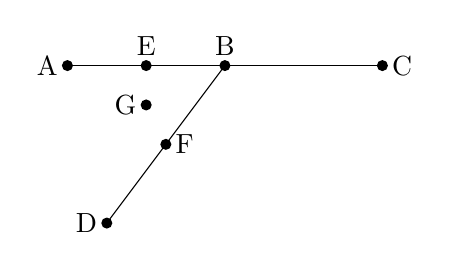
\begin{tikzpicture}

% Define coordinates for easier positioning
\coordinate (A) at (0,0);
\coordinate (B) at (2,0);
\coordinate (C) at (4,0);
\coordinate (D) at (0.5,-2);
\coordinate (E) at (1,0);
\coordinate (F) at (1.25,-1);
\coordinate (G) at (1,-0.5);

% Draw the lines
\draw (A) -- (C);
\draw (B) -- (D);


% Add the dots
\fill (A) circle (2pt) node[left] {A};
\fill (B) circle (2pt) node[above] {B};
\fill (C) circle (2pt) node[right] {C};
\fill (D) circle (2pt) node[left] {D};
\fill (E) circle (2pt) node[above] {E};
\fill (F) circle (2pt) node[right] {F};
\fill (G) circle (2pt) node[left] {G};

\end{tikzpicture}
    \begin{enumerate}
        \item Mid point of $AB$, $i\cdot e\cdot$ at point $E$
        \item Mid point of $BD$, $i\cdot e\cdot$ at point $F$
        \item Junction point $B$
        \item at a point $G$ lying within the area $ABC$
    \end{enumerate}
    \item Let $M_0$ be the total mass of a single rocket, $M_P$ be the total mass of propellant, $M_L$ be the mass of payload carried by the rocket and $M_S$ be the mass of inert structural components. If $I_{sp}$ is the specific impulse of the propulsion system \brak{in\,seconds} and $g$ is the acceleration  due to gravity, then the maximum velocity that can be attained by the rocket vehicle in absence of gravity and atmospheric drag is given by
    \begin{enumerate}
        \item $gI_{sp}\ln\brak{\frac{M_0}{M_P}}$
        \item $gI_{sp}\ln\brak{\frac{M_0}{M_L+M_P}-1}$
        \item $gI_{sp}\ln\brak{\frac{M_0}{M_S}}$
        \item $gI_{sp}\ln\brak{\frac{M_0}{M_0-M_P}}$
    \end{enumerate}
    \item An ideal axial compressor is driven by an ideal turbine across which the total temperature ratio is $0.667$. If the total temperature at turbine inlet is $T_0=1500\,K$ and specific heat of gas $c_p=1\,\frac{kJ}{kg}K$, the power drawn by the compressor per unit mass flow rate of air is approximately
    \begin{enumerate}
        \item $300\, \frac{kW}{kg}s$
        \item $1000\,\frac{kW}{kg}s$
        \item $600\,\frac{kW}{kg}s$
        \item $500\,\frac{kW}{kg}s$
    \end{enumerate}
    \item The performance of a solid rocket motor is improved by replacing the old propellant with the new one. The new propellant gives a combustion temperature $40\%$ higher than the previous propellant without appreciable change in molecular weight of combustion products and other operating parameters. By approximately what percentage is the specific impulse of the new motor higher than the old one?
    \begin{enumerate}
        \item $18\%$
        \item $96\%$
        \item $42\%$
        \item $112\%$
    \end{enumerate}
    \item A solid rocket motor has an end burning grain of cross-sectional area $A_{CS}=0.4\,m^2$. The density of propellant is $\rho_p=1500\,\frac{kg}{m^3}$ and has linear regression rate $r=5\,\frac{mm}{s}$. If the specific impulse of the propulsion system is $I_{sp}=200\,seconds$, the thrust  produced by the motor is approximately
    \begin{enumerate}
        \item $3\,kN$
        \item $6\,kN$
        \item $1.5\,kN$
        \item $12\,kN$
    \end{enumerate}
